\chapter{Nuclear Physics}
\begin{itemize}
    \item The Rutherford-Geiger-Marsden experiment.
    \begin{table}[H]
        \centering
        \begin{tabular}{ScSc}
            \toprule
            Observation & Explanation\\
            \midrule
            \begin{minipage}{0.35\textwidth}
                Most \(\alpha\)-particles passed straight through the foil, \emph{undeflected}.
            \end{minipage}& 
            \begin{minipage}{0.65\textwidth-50.4pt}
                An atom comprises of mostly empty space, with \emph{most of its mass concentrated in its nucleus which is very small in size \hly{compared} to the atom}. Hence, most pass through the empty space in the metal foil's atoms with minimal deflection.
            \end{minipage}\\
            \midrule
            \begin{minipage}{0.35\textwidth}
                Less than \hly{1\%} of the \(\alpha\)-particles were \emph{scattered backwards}, with an angle of \emph{deflection} exceeding \(90^\circ\).
            \end{minipage}& 
            \begin{minipage}{0.65\textwidth-50.4pt}
                Only a very small proportion of \(\alpha\)-particles --- that pass sufficiently close to or are incident on the nucleus of a metal foil atom --- experience \emph{strong repulsive electric forces} by the nucleus and are hence deflected by large angles\({}>90^{\circ}\).
            \end{minipage}\\
            \bottomrule
        \end{tabular}
        \caption{The Rutherford-Geiger-Marsden experiment: observations and explanations.}
        \label{table:rutherford-geiger-marsden}
    \end{table}
    \begin{example}{}{}
        In the \(\alpha\)-particle scattering experiment, only a small proportion of the \(\alpha\)-particles incident on the metal foil are deflected through angles greater than \(90^{\circ}\). \hspace*{\fill} [3]
        % \begin{itemize}
        %     \item An atom comprises of mostly empty space, with \emph{most of its mass concentrated in its nucleus which is very small in size compared to the atom}. Hence, most pass through the empty space in the metal foil's atoms with minimal deflection.
        %     \item Only a very small proportion of \(\alpha\)-particles --- that pass sufficiently close to or are incident on the nucleus of a metal foil atom --- experience \emph{strong repulsive electric forces} by the nucleus and are hence deflected by large angles\({}>90^{\circ}\).
        % \end{itemize}
    \end{example}
    \item[\AsteriskThin] A \emph{isotope} is one of two or more atoms with the \emph{same atomic number} but \emph{different number of neutrons}.
    \item[\AsteriskThin] The \emph{unified atomic mass unit} \(u\) is equivalent to \emph{one-twelfth} of the mass of a carbon-12 atom. i.e. 1 \(u=1.66\cdot 10^{-27}\) kg.
    \item[\AsteriskThin] The \emph{mass defect} is the amount by which the mass of an atomic \emph{nucleus} is less than the sum of the masses of its \emph{constituent particles}. i.e.
    \[\text{mass defect }\Delta m=\text{sum of masses of nucleons}-\text{mass of nucleus}.\]
    \item[\AsteriskThin] The \emph{binding energy} of a nucleus is the amount of energy that is required to \emph{break a nucleus} into its \emph{constituent nucleons}.
    \item Binding energy is not a form of stored energy. 
    \item Mass-energy equivalence: \(E=mc^2\).
    \item[\AsteriskThin] The \emph{binding energy per nucleon} is defined as the \emph{binding energy} of a nucleus divided by the \emph{number of nucleons} in the nucleus.
    \begin{figure}[H]
        \centering
        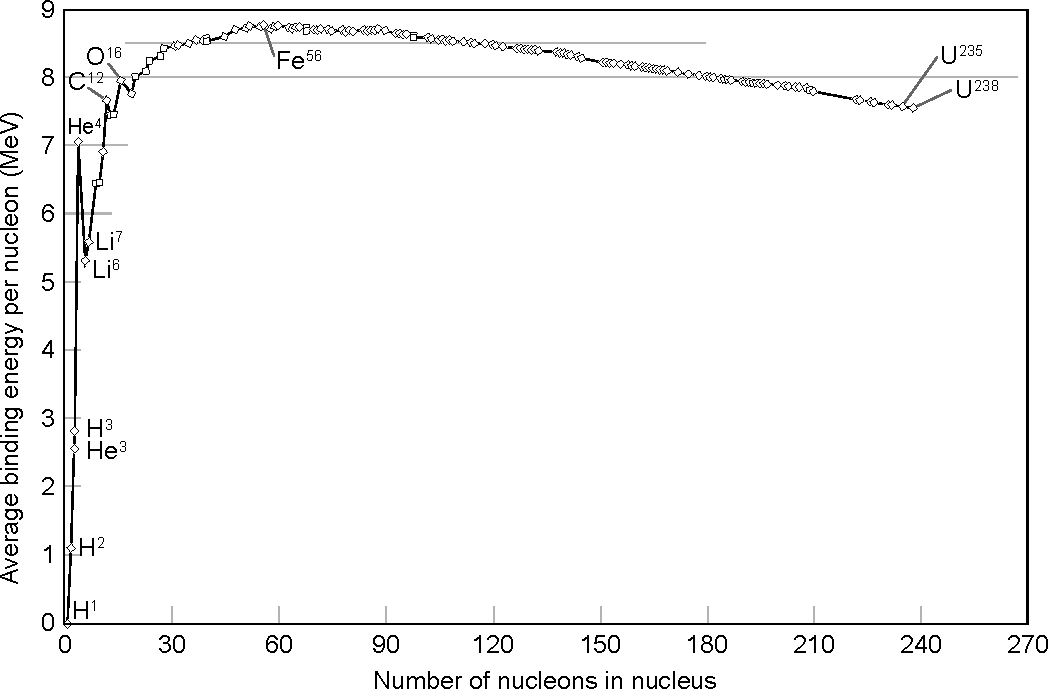
\includegraphics[width=0.81\textwidth]{../images/Binding energy per nucleon.pdf}
        \caption{\ref{source:binding-energy-per-nucleon} The variation of binding energy per nucleon with nucleon number.}
        \label{fig:binding-energy-per-nucleon}
    \end{figure}
    \item Remember that, Fe-56 has a binding energy per nucleon of 8.8 MeV and is located near (slightly to the right of) the peak.
    \item The binding energy per nucleon can be seen as a measure of stability: a higher binding energy per nucleon corresponds to a higher stability of the nucleus.
\end{itemize}
\begin{minipage}{0.5\textwidth}
    \begin{figure}[H]
        \centering
        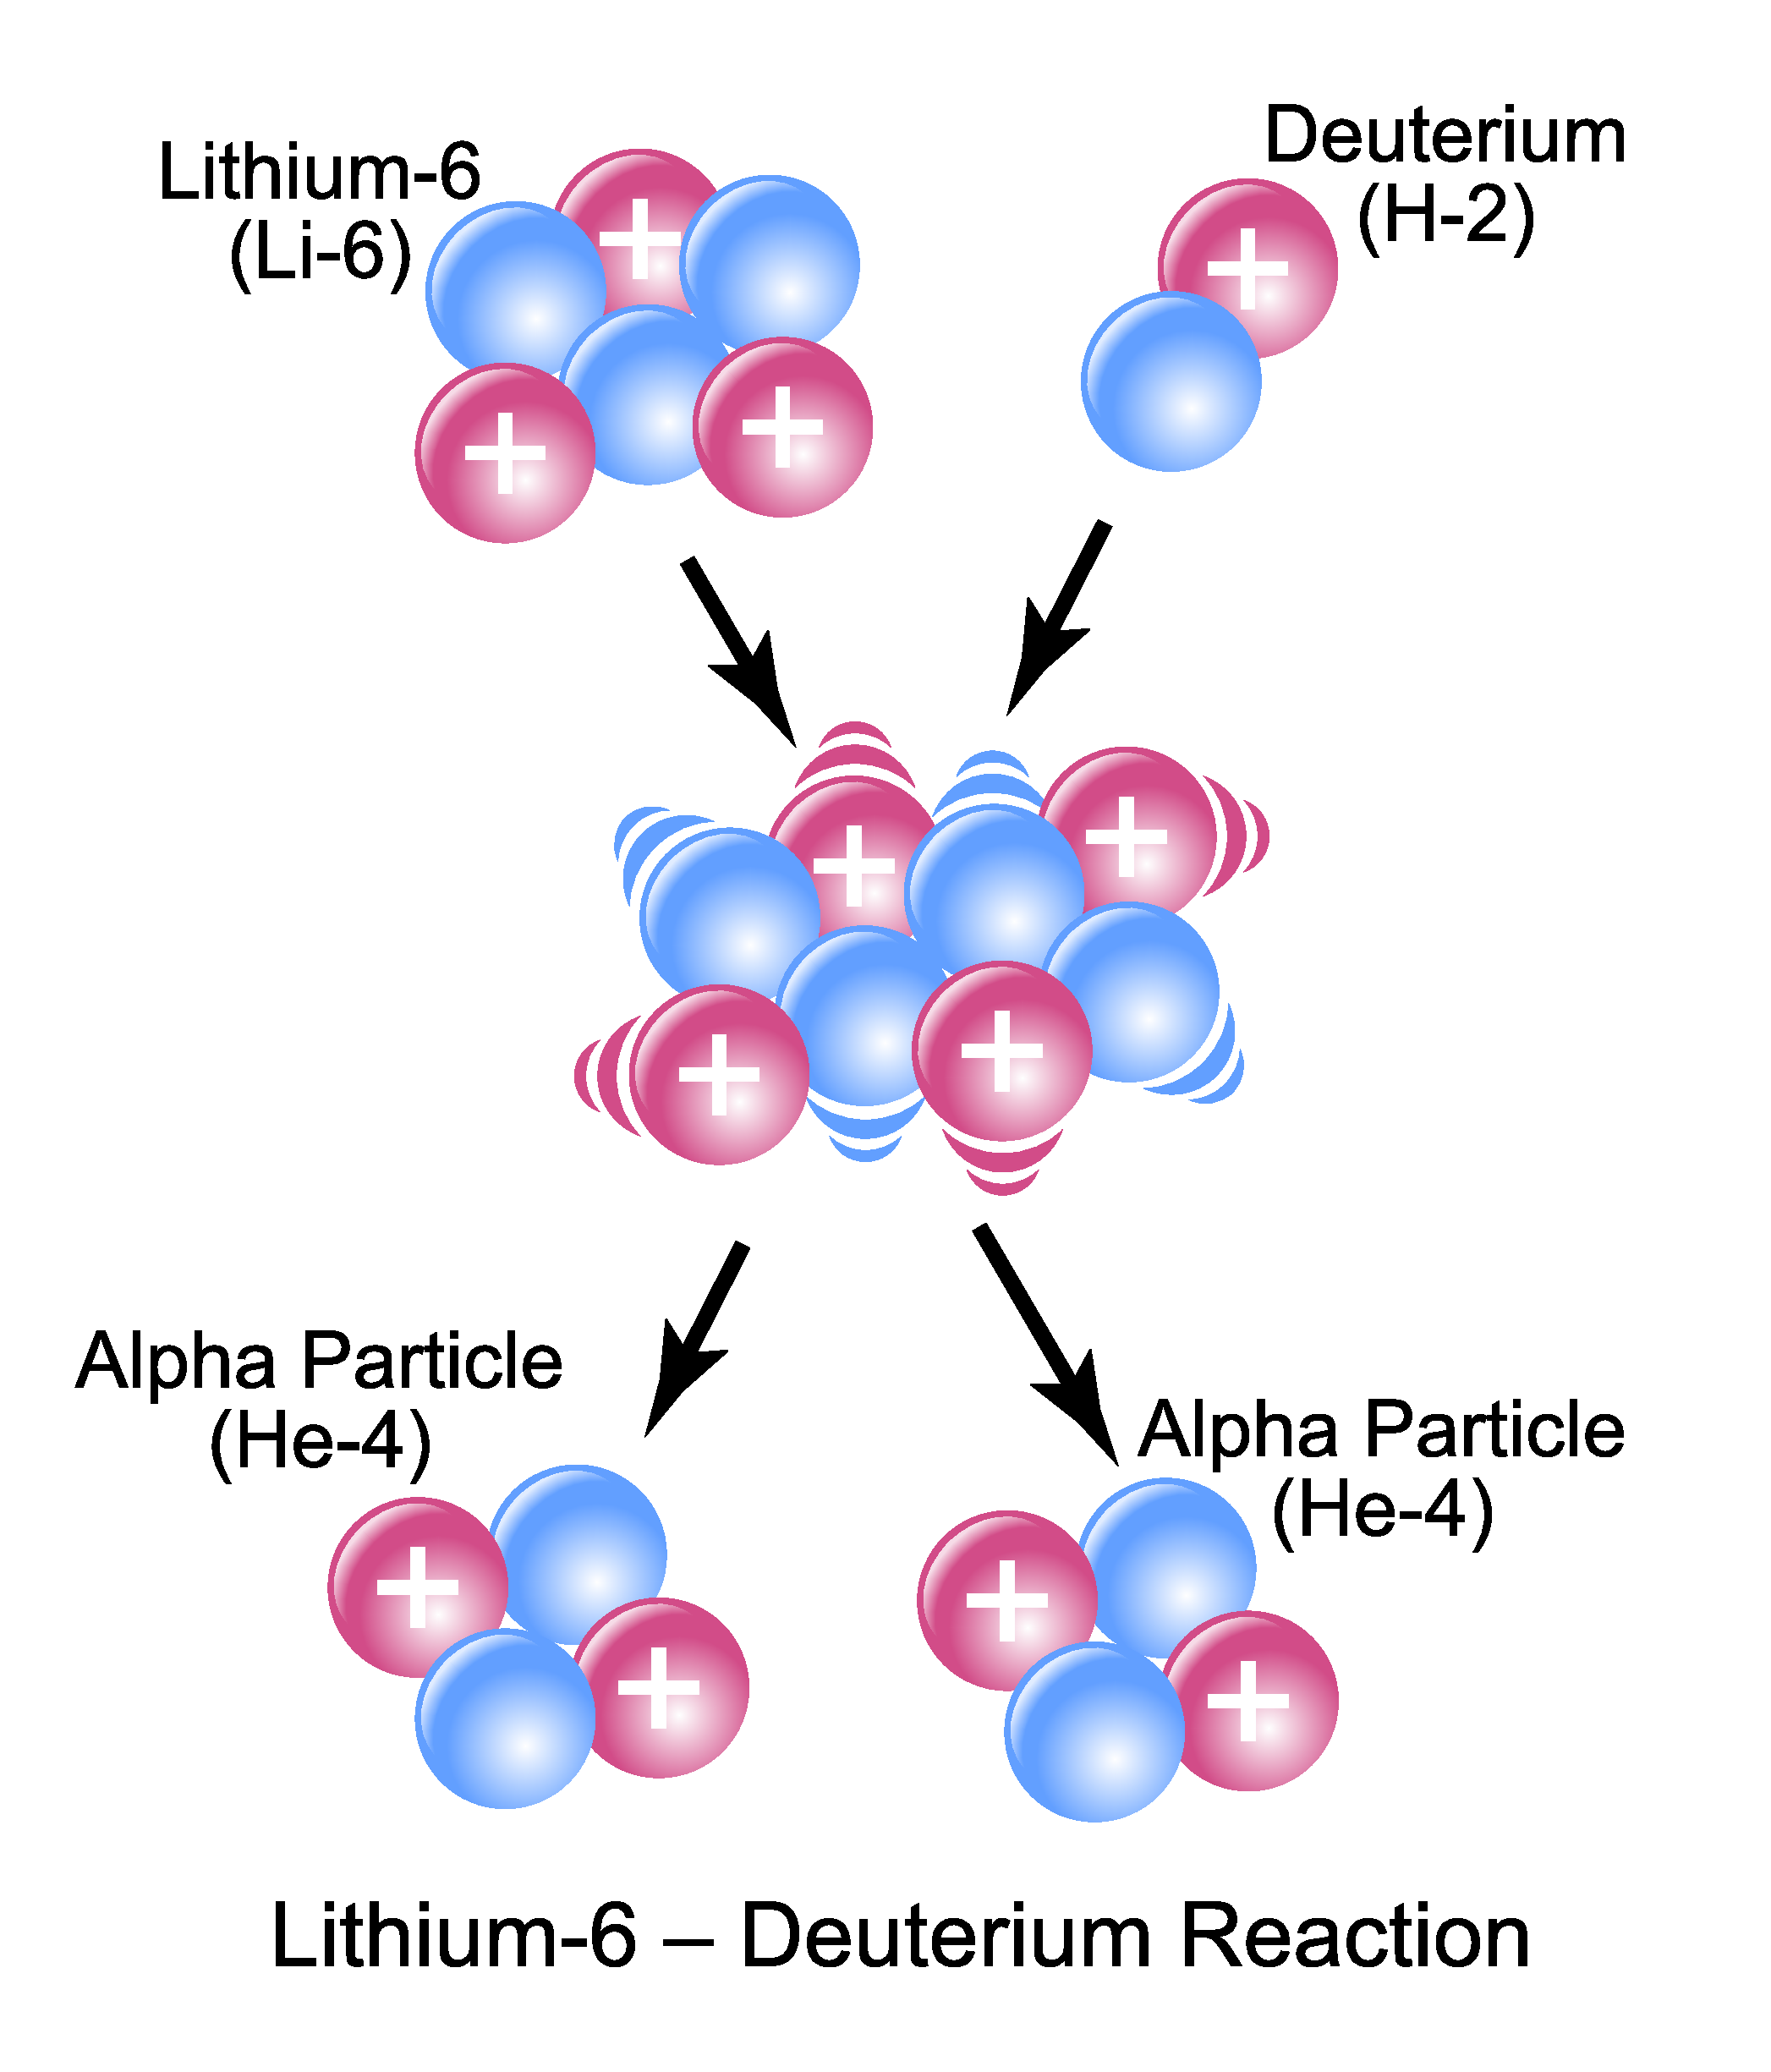
\includegraphics[width=\textwidth]{../images/Li6-D_Reaction.pdf}
        \caption{\ref{source:nuclear-fusion-and-fission} Nuclear fusion followed by fission.}
        \label{fig:nuclear-fusion-and-fission}
    \end{figure} 
\end{minipage}%
\begin{minipage}{0.5\textwidth}
    \begin{itemize}
        \item[\AsteriskThin] \emph{Nuclear fission} occurs when an atomic nucleus of greater mass splits into \emph{two} nuclei, each of \emph{smaller masses} and \emph{approximately} of the \emph{same nucleon number} as each other.
        \item[\AsteriskThin] \emph{Nuclear fusion} occurs when two nuclei of \emph{smaller nucleon numbers} fuse to form a single nucleus of a \emph{larger nucleon number}.
        \item Useful equations for calculating the energy liberated in a nuclear reaction. 
        \begin{enumerate}
            \item energy released\({}={}\)(mass of reactants\({}-{}\)mass of products)\({}c^2\).
            \item energy released\({}={}\)B.E. of products\({}-{}\)B.E. of reactants.
        \end{enumerate}
        \item Conserved quantities in nuclear reactions.
        \begin{enumerate}
            \item Nucleon number.
            \item Charge. The \emph{atomic numbers} of reactants and products each sum to the same total. \emph{But}, the total \emph{number of protons} may change due to beta decay. i.e. 
            \(\ce{_Z^A\text{X}}\to\ce{_{Z+1}^A\text{X}}+\ce{_{-1}^0\text{e}}\).
            \item Mass-energy.
        \end{enumerate}
    \end{itemize}
\end{minipage}
\begin{itemize}
    \item[\AsteriskThin] Radioactive decay is the \emph{spontaneous} and \emph{random} disintegration of atomic nuclei into another (nuclear) species through the \emph{emission} of alpha or beta particles or the de-excitation of nuclei to lower energy states through the emission of gamma radiation.
    \begin{itemize}
        \item \emph{Spontaneous} means that the nucleus decays because it is \emph{unstable}, not because of \emph{external conditions}.
        \item \emph{Random} means that it is impossible to predict \emph{which} nucleus will delay or \emph{when} a particular nucleus will decay.
    \end{itemize}
    \begin{example}{}{}
        State \emph{experimental evidence} to suggest that the process of radioactive decay is
        \begin{enumerate}
            \item random
            \item spontaneous.
        \end{enumerate}
        Answer:
        \begin{enumerate}
            \item When using a Geiger-Muller tube connected to a ratemeter, the count rate shown on the ratemeter shows unpredictable fluctuations that vary significantly each time the experiment is conducted.
            \item When using a Geiger-Muller tube connected to a ratemeter, the average count rate is not affected by external conditions such as temperature and pressure.
        \end{enumerate}
    \end{example}
    \item[\AsteriskThin] \emph{Background radiation} is the radiation detected by a \emph{radiation counter} when \emph{no radioactive source} is nearby.
    \item[\AsteriskThin] The \emph{activity} \(A\) of a radioactive isotope is defined as the number of \emph{nuclear disintegrations per unit time}.
    \item The count rate \(C\) is the rate at which counts are triggered on a ratemeter, by ionising radiation. 
    \item \emph{Note.} The count rate is \emph{not the same} as activity. In fact, \(C\leq A\) because not all emissions --- stemming from radioactive decay --- are counted. Some reasons include:
    \begin{enumerate}
        \item Not all the radiation is directed towards the detector.
        \item Some of the radiation will be absorbed in the source itself, and by the air between the source and the detector. 
    \end{enumerate}
    \item[\AsteriskThin] The \emph{decay constant} \(\lambda\) of a \emph{sample of a radioactive nuclide} is the \emph{probability} that a nucleus will \emph{decay per unit time}. 
    \item The number \(N\) of undecayed nuclei is such that \(A=-\frac{dN}{dt}=\lambda N\).
    \item The number \(N\) of undecayed nuclei, mass \(m\) of radioactive sample, activity \(A\), and count rate \(C\) all follow the equation \(y=y_0e^{-\lambda t}\) (\(y=N,m,A,C\)).
    \item When we are given a set of plotted points and asked to determine a value for half-life, do the following.
    \begin{itemize}
        \item Draw the curve of best-fit.
        \item Calculate two values for half-life and take their mean:
        \begin{itemize}
            \item[] Time to half count rate from \rule{0.5cm}{0.01mm} to \rule{0.5cm}{0.01mm}\({}=x\).
            \item[] Time to half count rate from \rule{0.5cm}{0.01mm} to \rule{0.5cm}{0.01mm}\({}=y\).
            \item[] Average half-life\({}=\frac{x+y}{2}=\rule{0.5cm}{0.01mm}\).
        \end{itemize}
    \end{itemize}
    \item[\AsteriskThin] The \emph{half-life} \(t_{1/2}\) of a \emph{radioactive isotope} is the \emph{average time} taken for its \emph{activity to be halved}. \emph{Note.} \(\lambda t_{1/2}=ln(2)\).
    \begin{example}{the importance of semantics.}{}
        A student defines half-life of a radioactive isotope as the \emph{time taken} for its activity to be halved. Explain why this is inappropriate. \hspace*{\fill} [2]
        \begin{itemize}
            \item Radioactive decay is a random process. \hspace*{\fill} [1]
            \item The time taken to decay by half will fluctuate; we should instead consider the \emph{average} time taken. \hspace*{\fill} [1]
        \end{itemize}
    \end{example}
    \begin{table}[H]
        \centering
        \begin{tabular}{ScScScScSc}
        % {|Sc|Sc|Sc;{2pt/2pt}Sc|Sc;{2pt/2pt}Sc|Sc|}
            \toprule
            Type of decay & Equation & Ionising power \textdownarrow & Penetration power \textuparrow & Velocity\\
            \midrule
            Alpha decay & 
            \begin{minipage}{3cm}
                \vspace{-4.07mm}
                \[\ce{_Z^A\text{X}}\to\ce{_{Z-2}^{A-4}\text{Y}}+\overbrace{\ce{_2^4\text{He}}}^{
                    \mathclap{
                        \alpha-\text{particle (zero electrons)\hspace{2.1cm}}}}
                        % \substack{\alpha-\text{particle}\\
                        % \text{(zero electrons)}}}}
                \]
            \end{minipage}&
            \begin{minipage}{2cm}
                \centering
                Strong

                (\(10^5\) ions per cm)
            \end{minipage}&
            \begin{minipage}{2cm}
                \centering
                Stopped by a few cm of air or paper 
            \end{minipage}& 
            \begin{minipage}{3cm-23pt}
                \centering
                \(10^7\text{ ms}^{-1}\) or 
                
                \(0.1c\)
            \end{minipage}\\
            \midrule
            Beta decay & 
            \begin{minipage}{3cm}
                \vspace{-4.07mm}
                \[\ce{_Z^A\text{X}}\to\ce{_{Z+1}^A\text{Y}}+\overbrace{\ce{_{-1}^0\text{e}}}^{
                    \mathclap{\beta-\text{particle}}\hspace{3mm}}\]
            \end{minipage}&
            \begin{minipage}{2cm}
                \centering
                (\(10^3\) ions per cm)
            \end{minipage}&
            \begin{minipage}{2cm}
                \centering
                5 mm of aluminum 
            \end{minipage}& 
            \begin{minipage}{3cm-23pt}
                \centering
                Continuous range up to 
                
                \(10^8\text{ ms}^{-1}\) or 
                
                \(0.9c\)
            \end{minipage}\\
            \midrule
            Gamma decay & 
            \begin{minipage}{3cm}
                \vspace{-4.07mm}
                \[\rule{0.5cm}{0.05mm}\to \rule{0.5cm}{0.05mm}+\overbrace{\ce{_0^0\gamma}}^{
                    \mathclap{\gamma-\text{ray}}}\]
            \end{minipage}& 
            \begin{minipage}{2cm}
                \centering
                Weak

                (indirect ionisation)
            \end{minipage}&
            \begin{minipage}{2cm}
                \centering
                Several cm of lead
            \end{minipage}& \(c\)\\
            \bottomrule
        \end{tabular}
        \caption{Types of radioactive decay.}
        \label{table:types-of-radioactive-decay}
    \end{table}
    % \begin{table}[H]
    %     \centering
    %     \begin{tabular}{|Sc|Sc|Sc;{2pt/2pt}Sc|Sc;{2pt/2pt}Sc|Sc|}
    %         \hline
    %         Type of decay & Equation & \multicolumn{2}{Sc|}{Ionising power} & \multicolumn{2}{Sc|}{Penetration power} & Velocity\\
    %         \hline
    %         Alpha decay & 
    %         \begin{minipage}{3cm}
    %             \vspace{-4.07mm}
    %             \[_Z^A\text{X}\to{}_{Z-2}^{A-4}\text{Y}+\overbrace{_2^4\text{He}}^{
    %                 \mathclap{
    %                     \alpha-\text{particle (zero electrons)\hspace{2.1cm}}}}
    %                     % \substack{\alpha-\text{particle}\\
    %                     % \text{(zero electrons)}}}}
    %             \]
    %         \end{minipage}&
    %         \multirow{3}{*}{\(\xdownarrow{1.5cm}\)} & 
    %         \begin{minipage}{2cm}
    %             \centering
    %             Strong

    %             (\(10^5\) ions per cm)
    %         \end{minipage}& \multirow{3}{*}{\(\xuparrow{1.5cm}\)} & 
    %         \begin{minipage}{2cm}
    %             \centering
    %             Stopped by a few cm of air or paper 
    %         \end{minipage}& 
    %         \begin{minipage}{3cm-23pt}
    %             \centering
    %             \(10^7\text{ ms}^{-1}\) or 
                
    %             \(0.1c\)
    %         \end{minipage}\\
    %         \cline{1-2}
    %         \cline{4-4}
    %         \cline{6-7}
    %         Beta decay & 
    %         \begin{minipage}{3cm}
    %             \vspace{-4.07mm}
    %             \[_Z^A\text{X}\to{}_{Z+1}^A\text{Y}+\overbrace{_{-1}^0\text{e}}^{
    %                 \mathclap{\beta-\text{particle}}\hspace{3mm}}\]
    %         \end{minipage}&
    %         &
    %         \begin{minipage}{2cm}
    %             \centering
    %             (\(10^3\) ions per cm)
    %         \end{minipage}&& 
    %         \begin{minipage}{2cm}
    %             \centering
    %             5 mm of aluminum 
    %         \end{minipage}& 
    %         \begin{minipage}{3cm-23pt}
    %             \centering
    %             Continuous range up to 
                
    %             \(10^8\text{ ms}^{-1}\) or 
                
    %             \(0.9c\)
    %         \end{minipage}\\
    %         \cline{1-2}
    %         \cline{4-4}
    %         \cline{6-7}
    %         Gamma decay & 
    %         \begin{minipage}{3cm}
    %             \vspace{-4.07mm}
    %             \[\rule{0.5cm}{0.05mm}\to \rule{0.5cm}{0.05mm}+\overbrace{_0^0\gamma}^{
    %                 \mathclap{\gamma-\text{ray}}}\]
    %         \end{minipage}&& 
    %         \begin{minipage}{2cm}
    %             \centering
    %             Weak

    %             (indirect ionisation)
    %         \end{minipage}&& 
    %         \begin{minipage}{2cm}
    %             \centering
    %             Several cm of lead
    %         \end{minipage}& \(c\)\\
    %         \hline
    %     \end{tabular}
    %     \caption{Types of radioactive decay.}
    %     \label{table:types-of-radioactive-decay}
    % \end{table}
    \begin{example}{}{}
        The isotope beryllium-7 is radioactive with a half-life of 53 days. A beryllium-7 nucleus decays by the emission of a \(\gamma\)-ray photon. State why, although the beryllium-7 is radioactive, the number of beryllium-7 nuclei in the sample does not change. \hspace*{\fill} [2]
        \begin{itemize}
            \item  The \(\gamma\)-ray photon emitted in the decay of a beryllium-7 nucleus is a quantum of energy that contains no protons or neutrons. \hspace*{\fill} [1]
            \item So the daughter nucleus is still a beryllium-7 nucleus. Hence, the number of beryllium-7 nuclei is constant. \hspace*{\fill} [1]
        \end{itemize}
    \end{example}
\end{itemize}
    \begin{minipage}{0.5\textwidth}
        \begin{figure}[H]
            \centering
            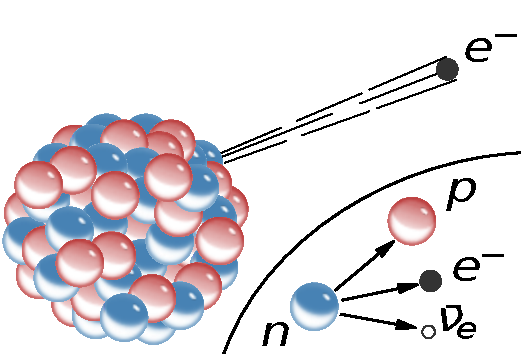
\includegraphics[width=\textwidth]{../images/Beta-minus_Decay.pdf}
            \caption{\ref{source:beta-decay} Beta decay.}
            \label{fig-beta-decay}
        \end{figure}
    \end{minipage}%
    \begin{minipage}{0.5\textwidth}
        \begin{itemize}
            \item In a beta decay, a \emph{neutrino} is emitted along with the \(\beta\)-particle, carrying away some kinetic energy and momentum. Hence, the electron emission may not be collinear, in the opposite direction of, the recoil of the nucleus.
            \item While a couple mm or cm of metal suffices to stop \(\beta\)-particles, X-rays (bremsstrahlung) may be produced outside the container: 
        \end{itemize}
    \end{minipage}
\begin{itemize}
    \item[]
        \begin{itemize}
            \item When \(\beta\)-particles --- electrons moving at \emph{high speeds} --- pass by the positively charged aluminum nuclei, they experience a sudden, \emph{large} deceleration. 
            \item The kinetic energy of the \(\beta\)-particles are lost through the emission of Bremsstrahlung X-ray photons.  
            \item X-ray photons have a higher penetrating power than \(\beta\)-particles. So, while \(\beta\) particles are absorbed, X-ray photons pass through the aluminum walls.
        \end{itemize}
        So, thicker layers of lower atomic mass materials --- plastic, wood, water, etc --- may be preferable.
    \item Biological effects of radiation.
    \begin{itemize}
        \item Direct effects. When radiation interacts with DNA, affecting (or even breaking) the bonds within, it impacts the ability of a cell to reproduce and survive. Mutations may also occur, eventually leading to cancer.
        \item Indirect effects. When radiation interacts with and breaks the bonds in water molecules, it creates free radicals: molecules which are highly reactive due to the presence of unpaired electrons. These free radicals form compounds which initiates harmful chemical reactions within cells, causing them to be destroyed.
    \end{itemize}
\end{itemize}
\begin{example}{}{}
    Explain why, although the count rates are too low for the radiation to cause immediate symptoms in the student, careful shielding of the source is still necessary.
    \begin{itemize}
        \item Ionising radiation damages DNA and causes biological harm to the body. Even though no immediate symptoms may arise, biological damage can build up with \emph{prolonged close-proximity} exposure. In the long run, the student might experience increased risk of cancer, among other health impacts.
        \item It also prevents radioactive contamination due to accidental inhalation or ingestion of the residues of the radioactive source --- especially if especially if the source is powdery --- which may lead to irreversible long run exposure to radioactive material.
    \end{itemize} 
\end{example}
\begin{example}{radioactive dating.}{}
    To find the age of a relic, a recreation of it is made. Suppose that 
    \begin{enumerate}
        \item The recreation is perfect. i.e. it is identical to the relic when it was first made.
        \item The background count rate has remained constant throughout time at \(C_B\).
        \item The only radioactive process that has affected the relic in its entire lifetime is \(\ce{_Z^A\text{X}}\to\ce{_{\mathcal{Z}}^{\mathcal{A}}\text{Y}}+\dots\)
        \item The number of \(\ce{_{\mathcal{Z}}^{\mathcal{A}}\text{Y}}\) nuclei only changes due to the reaction \(\ce{_Z^A\text{X}}\to\ce{_{\mathcal{Z}}^{\mathcal{A}}\text{Y}}+\dots\)
    \end{enumerate}
    \begin{enumerate}[label=(\alph*)]
        \item In the absence of other radioactive samples, the relic and its recreation are found to have count rate \(C'\) and \(C\) respectively. Find the age \(T\) of the relic, in terms of the half life \(t_{1/2}\) of \(\ce{_Z^A\text{X}}\). 
        \begin{align*}
            C&=C_0e^{-\lambda t}\\
            C'&=Ce^{-\frac{T\ln(2)}{t_{1/2}}}\\
            T&=\frac{\ln(C/C')}{\ln(2)}\cdot t_{1/2}.
        \end{align*}
        \item The ratio of \(\ce{_Z^A\text{X}}\) to \(\ce{_{\mathcal{Z}}^{\mathcal{A}}\text{Y}}\) for the relic and its recreation are \(k'\) and \(k\), respectively. Find the age \(T\) of the relic.

        \vspace{0.5\baselineskip} Let \(M\) denote the initial number of \(\ce{_{\mathcal{Z}}^{\mathcal{A}}\text{Y}}\) nuclei. Since \(N_0/M=k\), we have \(M=N_0/k\). Therefore,
        \begin{align*}
            \frac{N}{M+(N_0+N)}&=k'\\
            \frac{N}{(1/k+1)N_0-N}&=k'\\
            (k'+1)N&=k'(1/k+1)N_0\\
            N_0e^{-\frac{T\ln(2)}{t_{1/2}}}&=\frac{k'(1/k+1)}{k'+1}\cdot N_0\\
            T&=\frac{t_{1/2}}{\ln(2)}\cdot\ln\left( \frac{k'+1}{k'(1/k+1)} \right).
        \end{align*}
        \item What are some limitations of radioactive dating?
        \begin{itemize}
            \item It cannot be used for very old samples, as the activity will be very low so the calculated age may not be accurate.
            \item We are assuming that the recreation has the same number of \(\ce{_Z^A\text{X}}\) and \(\ce{_{\mathcal{Z}}^{\mathcal{A}}\text{Y}}+\dots\) nuclei as the relic when it was first made.

            (The exact assumption depends on the question. It might instead be the concentration of \(\ce{_Z^A\text{X}}\) to \(\ce{_Z^{\mathcal{A}}\text{X}}\), instead of the exact number.)
            \item It cannot be used for living things, if \(\ce{_Z^A\text{X}}\) or \(\ce{_{\mathcal{Z}}^{\mathcal{A}}\text{Y}}+\dots\) is carbon-14.

            (Living things will continue to absorb carbon-14 from their surroundings into their tissue. This process stops, allowing the number/concentration of carbon-14 to decrease, only after death.)
            \item[\emph{Note.}] Chemical processes do not change the \emph{ratio} of two isotopes; both are used in equal proportions as the chemical behavior of isotopes are nearly identical. 
        \end{itemize}
    \end{enumerate}
\end{example}